\documentclass[12pt]{article}
\usepackage[english]{babel}
\usepackage{natbib}
\usepackage{url}
\usepackage[utf8x]{inputenc}
\usepackage{amsmath}
\usepackage{graphicx}
%\graphicspath{{img/}} .md doesn't understand this and have problems
\usepackage{parskip}
\usepackage{fancyhdr}
\usepackage{vmargin}
\usepackage{xcolor}

\usepackage[table,xcdraw]{xcolor}
\setmarginsrb{3 cm}{2.5 cm}{3 cm}{2.5 cm}{1 cm}{1.5 cm}{1 cm}{1.5 cm}


\makeatletter
\let\thetitle\@title

\let\thedate\@date
\makeatother

\pagestyle{fancy}
\fancyhf{}
\rhead{\theauthor}
\lhead{\thetitle}
\cfoot{\thepage}

\begin{document}

%%%%%%%%%%%%%%%%%%%%%%%%%%%%%%%%%%%%%%%%%%%%%%%%%%%%%%%%%%%%%%%%%%%%%%%%%%%%%%%%%%%%%%%%%

\begin{titlepage}
	\centering
    
    
\includegraphics[scale = 0.75]{img/Logo.png} \\[1.0 cm]
    
    \vspace{4 cm}
    
    {\LARGE Experiment report} \\[0.2 cm]
    
    \vspace{1 cm}
    
    \rule{\linewidth}{0.2 mm} \\[0.4 cm]
    
	\textsc{\LARGE Ethereum vs. Hyperledger}\\[0.2 cm]
	\textsc{\lARGE Comparison of throughput for non-conflicting transactions} \\[0.2 cm]
	\rule{\linewidth}{0.2 mm} \\[0.4 cm]
	
	{\huge \bfseries \thetitle}\\
	
	\vspace{2 cm}
	
	\begin{minipage}{0.4\textwidth}
		
		\begin{flushleft} 
			\emph{Authors:} \\
			Jacek Janczura \linebreak
			Igor Molcean \linebreak
			Julian Valentino Weigel \linebreak
			Kim Janik Jasun Herter
		\end{flushleft}
	\end{minipage}\\[2 cm]
	

 
	\vfill
	
\end{titlepage}

%%%%%%%%%%%%%%%%%%%%%%%%%%%%%%%%%%%%%%%%%%%%%%%%%%%%%%%%%%%%%%%%%%%%%%%%%%%%%%%%%%%%%%%%%

\tableofcontents
\pagebreak

%%%%%%%%%%%%%%%%%%%%%%%%%%%%%%%%%%%%%%%%%%%%%%%%%%%%%%%%%%%%%%%%%%%%%%%%%%%%%%%%%%%%%%%%%

\begin{abstract}
In this experiment, we compared Ethereum and Hyperledger private networks with regard to throughput for non-conflicting transactions, i.e. transactions that do not cause double-spending. We proposed two mathematical definitions of throughput and used them to compare both systems. We set up the networks in similar conditions and provided them with synthetically generated workload. We used custom tools to collect relevant data from systems’ logs. Finally, we came to the conclusion that Ethereum, generally, shows more promising results. However, further research will be needed for more profound analysis.
\end{abstract}

\newpage
\section{Introduction}
%\textit{Authors: Jacek Janczura, Igor Molcean, Kim Janik Jasun Herter, Julian Weigel (Proof-of-Stake part)}

Blockchain is a relatively new concept. It represents a distributed, uncentralized and immutable data storage where every single change can be seen by anyone and the whole amount of data is stored at every node that participates in the network. This makes blockchain quite different from traditional databases that try to restrict access as far as possible and require centralized coordinator for replication. Unlike many distributed storages, blockchain does not use redundancy to increase performance but rather to improve resilience of the system. For the first time, the term was used in context of Bitcoin in 2008 \cite{bitcoin}. This became the reason why blockchain is often associated with cryptocurrencies but potencial of this technology is actually much higher.

One of the big problems that prevents blockchain-based technologies from entering our everyday life is limited throughput. For example, limited block size in case of Bitcoin, caused the so-called "Bitcoin scalability problem" which resulted in intense research \cite{bitcoin_scaling} and numerous proposals on how to increase throughput of the system. Being able to perform operations fast, is important for a system that is used by big number of people worldwide, this is why throughput becomes so critical in context of blockchain systems.

The goal of our experiment is to measure the throughput for two widely used blockchain systems, Ethereum and Hyperledger, in order to learn how effective their underlying algorithms process big numbers of submitted transactions in short periods of time.

\subsection{Main concepts}

\textbf{Throughput} is the maximum rate at which transactions can be successfully processed by the blockchain, i.e. end up in a block of the canonical chain. Not to be confused with \textbf{Bandwidth}, which is the maximum possible rate at which transactions can be processed theoretically. Both are measured in transactions per second (Tx/s).

\textbf{Proof-of-Authority} is an algorithm where only authorized nodes, called sealers or signers, can add blocks to chain. To make sure a malicious node can’t do harm to the network, any signer can sign at most one of a number $\lfloor S/2 \rfloor + 1$ of consecutive blocks (where $S$ is the number of sealers). PoA algorithm used in Ethereum is called Clique \cite{clique}.

\textbf{Proof-of-Stake} is a consensus algorithm where decisions are made based on weighted random choice. It is calculated by participation duration in combination with the size of the stake. It’s byzantine fault tolerant \cite{pos}.


\section{Method}
%\textit{Authors: Igor Molcean, ... (Hyperledger-specific parts)}

This sections will describe materials and procedures that were used during the experiment. We will start with formal mathematical definition of the main metric, continue with the experimental set up and finish with procedures for data collection.

\subsection{Transaction throughput} \label{throughput}
In out experiment, we defined throughput as average number of transactions in a block divided by the block frequency:

$$Throughput = \frac{1/N \sum_{b=1}^{N} T_b}{F}$$

where
\begin{itemize}
    \item $N$ is total number of transactions submitted
    \item $T_b$ is number of transactions contained in block $b$
    \item $F$ is block frequency
\end{itemize}

Other definitions can also be found in literature. We decided to compare one of them with ours. It is formulated as follows: transaction throughput is the rate at which valid transactions are committed by the blockchain System Under Test (further SUT) in a defined time period \cite{hyperledger_paper}. This definition may be presented as the following formula:

$$Throughput_{alt} = \frac{N}{t_{b_N} - t_{T_0}}$$

where
\begin{itemize}
    \item $N$ is total number of submitted transactions submitted
    \item $t_{b_N}$ is the commit time of the last block
    \item $t_{T_0}$ is the submission time of the initial transaction
\end{itemize}

\subsection{Experimental set up}

The experimental setup consists of the two private blockchain networks deployed in a controlled distributed environment. As such environment we used several Amazon AWS EC2 instances, their parameters are presented in table \ref{instance_params}. Each node runs on its own Virtual Machine (further VM) but all VMs are located in the same subnetwork to minimize the effect of network latencies to the experiment. For simplicity, both networks were deployed with just one mining node. We conducted the same experiment several times with different values of $N$.

\begin{table}[ht]
    \centering
    \begin{tabular}{|l|l|l|l|l|}
        \hline
        Type & Cores & CPU & RAM & Network performance \\
        \hline
        t2.micro & 1 & 3.3 GHz & 1 GiB & Low to Moderate \\
        \hline
    \end{tabular}
    \caption{Parameters of the EC2 instances \cite{ec2_params}}
    \label{instance_params}
\end{table}

In case of Ethereum, we created a private network with the Proof-of-Authority consensus algorithm. There are 2 nodes running on Geth \cite{geth}: Node 1 is sealing blocks and Node 2 is submitting party-to-party transactions to the blockchain. In order to enable nodes’ communication, we used the so-called Bootnode \cite{bootnode}. The block frequency $F$ was set to 2 seconds. In order to guarantee that all transactions are non-conflicting, i.e. do not potentially cause double spending, we preallocated enough Ether on the account used as a transaction sender.

Additionally we have tested another mining setup. In that second experimental version ETH block period was setup to 0. That means that miner starts to mine a new blocks only When there are a new transactions. If there are no transactions in a blockchain mining frequency drops to 0 and the mining nodes wait for the new transaction to be authorised and added to the blockchain. 

{\color{red} Hyperledger}



\subsection{Methods of data collection}
In case of Ethereum, all necessary data could be found directly in the logs generated by Geth. For this purpose, we developed a parser that went through the log files extracting relevant information and storing it in a CSV file. By relevant information, we mean the number of transactions for each block ($T_b$) as well as timestamps of the first submitted transaction ($t_{T_0}$) and last committed block ($t_{b_N}$). Knowing block frequency ($F$), total number of transactions ($N$) and being able to parse everything else, it became trivial to calculate throughput according to the definitions presented in subsection \ref{throughput}.

{\color{red} Hyperledger}



\section{Results}
%\textit{Authors:}

 Blockchain is not a normal BASE or ACID database, where transactions are executed immediately after submitting. In case of blockchain transactions are stored in a blocks and than commonly added to a blockchain.
 As it is clearly visible in a Table \ref{table:2} measuring throughput for the number of transactions less then the block capacity is pointless. That is why we present AVG filtered values where we do not include the measurements for $tx < 500$.

\subsection{ETH measurements with block mining period 2s.}
Throughput was measured consequently with a two previously aforementioned definitions. In the Fig.\ref{fig:throughput1} throughput was measured as average number of transactions in a block divided by the block frequency and in the Fig.\ref{fig:throughput2} throughput was measured using our own formula. 

\begin{table}[h]
\begin{tabular}{l|l|l|l|l|}
\hline
\multicolumn{1}{|l|}{\textbf{tx}} & \textbf{tbn-t0 {[}s{]}} & \textbf{Thr. alt. {[}tx/s{]}} & \textbf{Avg(tx/block)} & \textbf{Thr. {[}tx/s{]}} \\ \hline
\multicolumn{1}{|l|}{\textit{10}} & \textit{2.69} & \textit{3.72} & \textit{10} & \textit{5} \\ \hline
\multicolumn{1}{|l|}{\textit{100}} & \textit{2.79} & \textit{35.80} & \textit{100} & \textit{50} \\ \hline
\multicolumn{1}{|l|}{\textit{1000}} & \textit{10.67} & \textit{93.72} & \textit{200} & \textit{100} \\ \hline
\multicolumn{1}{|l|}{\textit{10000}} & \textit{99.82} & \textit{100.18} & \textit{204.08} & \textit{102.04} \\ \hline
\multicolumn{1}{|l|}{\textit{100000}} & \textit{1711.73} & \textit{58.42} & \textit{117.1} & \textit{58.55} \\ \hline
\multicolumn{1}{|l|}{\textit{489290}} & \textit{8935.53} & \textit{54.76} & \textit{109.53} & \textit{54.765} \\ \hline
 & \textbf{AVG} & \textit{\textbf{57.77}} & \textit{\textbf{123.45}} & \textit{\textbf{61.73}} \\ \cline{2-5} 
 & \textbf{AVG filtered} & \textit{\textbf{76.77}} & \textit{\textbf{157.68}} & \textit{\textbf{78.84}} \\ \cline{2-5} 
\end{tabular}
\caption{ETH: Throughput measurement results. Block mined every 2s.}
\label{table:2}
\end{table}

Table \ref{table:2} presents the results of the throughput measurements. In ethereum private blockchain we have observed that in case of lower blockchain load ($tx < 10000$) throughput is in average around 100 transactions per second and the average number of transactions in a block is then on the level around 200 tx/block. Unfortunately in case of higher blockchain load  throughput falls to the level of 50 tx/s and stays on that level even in a really overloaded blockchain. 


 
The results from measuring the throughput in both ways results in a similar numbers - average filtered throughput between 75-80 tx/s. 

\begin{figure}[h]
    \centering
    %\captionsetup{justification=centering}
    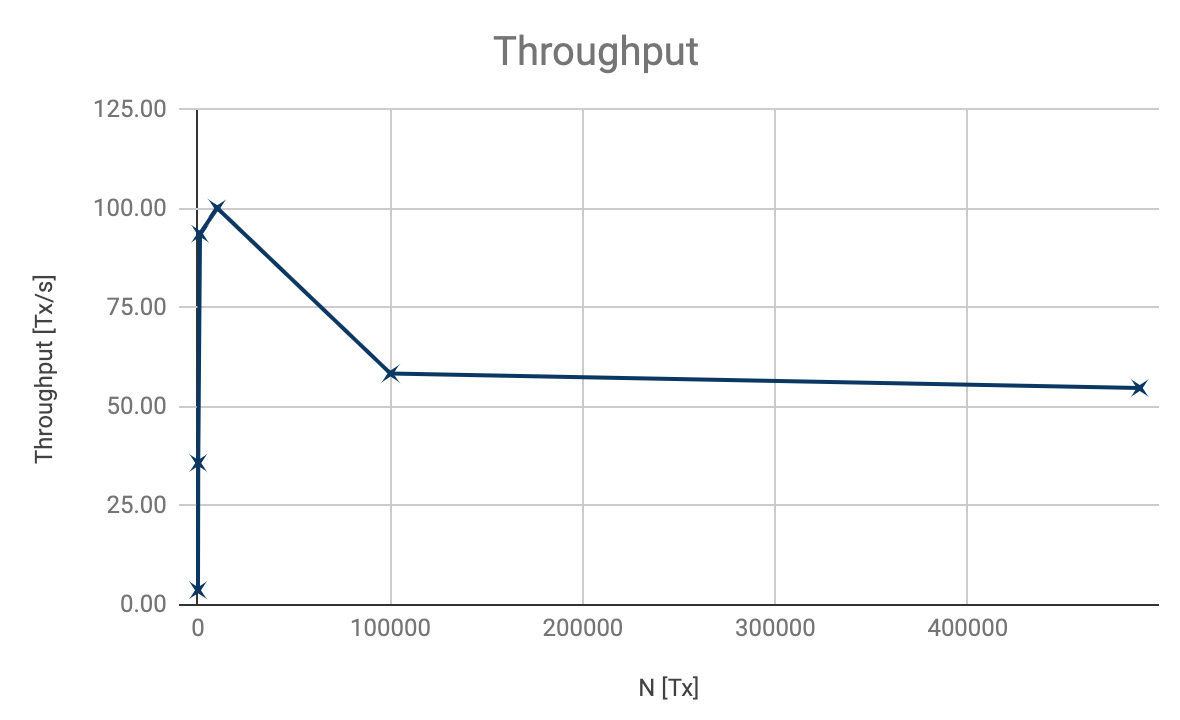
\includegraphics[width=0.9\textwidth]{img/Throughput_ETH.png}
    \caption{ETH: Throughput as average number of transactions in a block divided by the block frequency}
    \label{fig:throughput1}
\end{figure}

\begin{figure}[h]
    \centering
    %\captionsetup{justification=centering}
    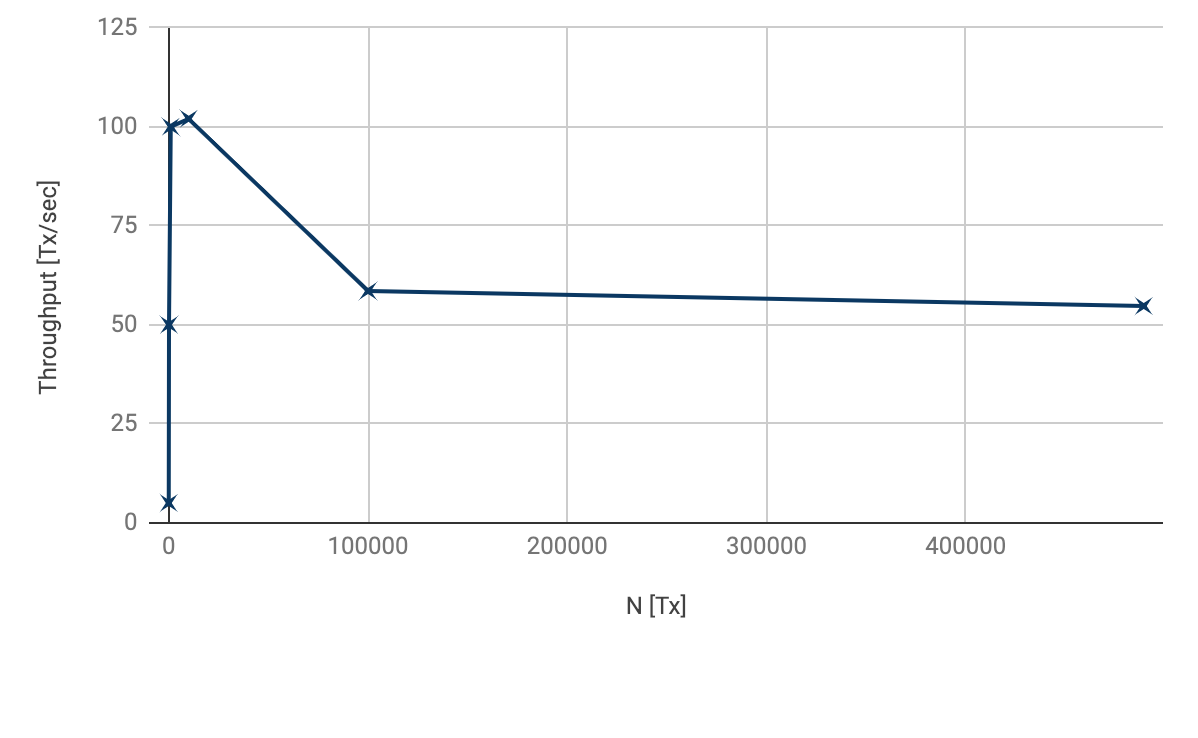
\includegraphics[width=0.9\textwidth]{img/Throughputalt.png}
    \caption{ETH: Throughput as total number of transactions divided by time from submitting the first transaction until mining the last block}
    \label{fig:throughput2}
\end{figure}

In a Fig. \ref{fig:txbig} we present the number of transactions per block. It is clearly visible that average tx/block stays in the level of 100 ts/block. We have as well data for 1 milion of transactions. The results are the same as for 100 000 but the chart is less clear that is why we have decided to present more clear chart.





\begin{figure}[h]
    \centering
    %\captionsetup{justification=centering}
    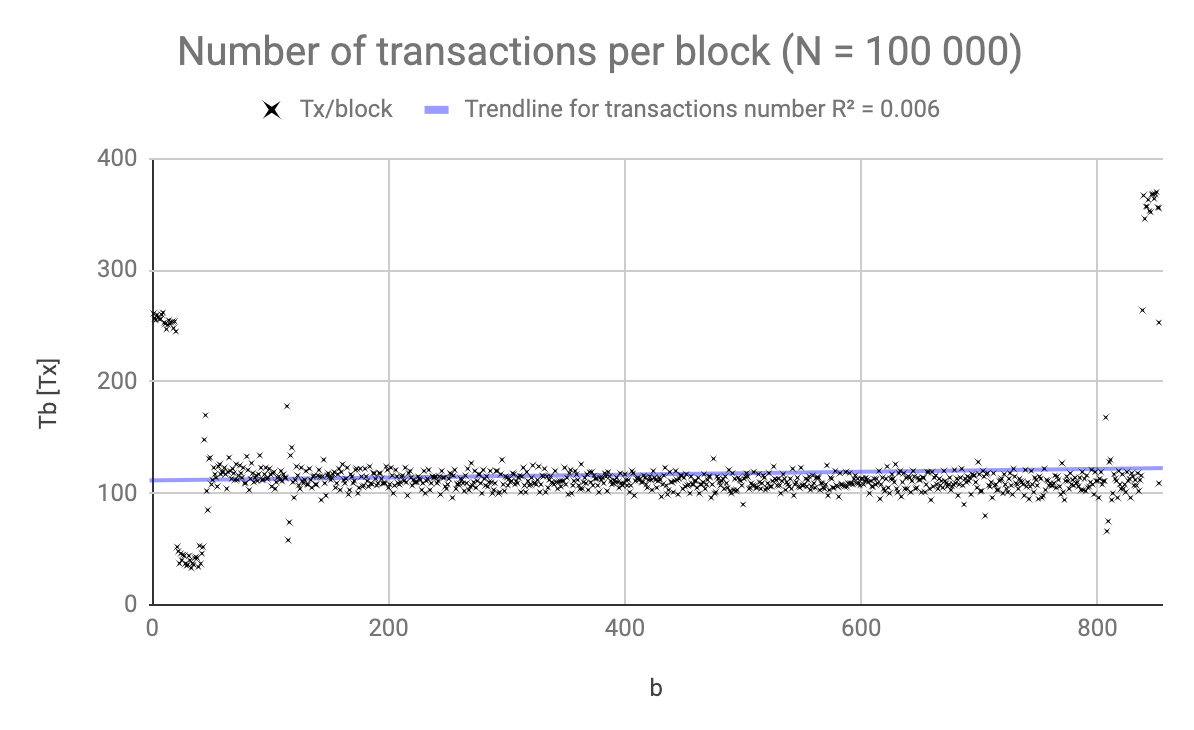
\includegraphics[width=0.9\textwidth]{img/txmed.png}
    \caption{ETH: Visualisation of taint analysis}
    \label{fig:txbig}
\end{figure}

\begin{figure}[h]
    \centering
    %\captionsetup{justification=centering}
    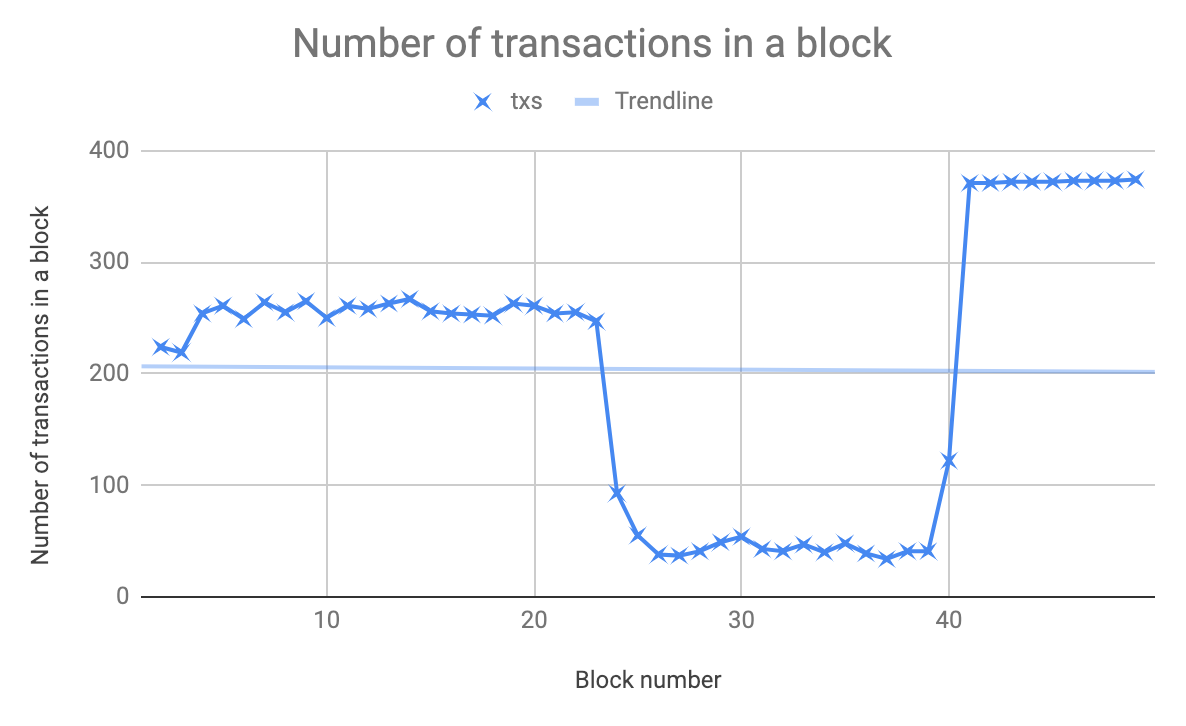
\includegraphics[width=0.9\textwidth]{img/TxNumperBlockSmall.png}
    \caption{ETH: Visualisation of taint analysis}
    \label{fig:txsmall}
\end{figure}

\subsection{ETH measurements with block mining period 0s.}
\subsection{Hyperledger}

\section{Future scope}
%\textit{Authors:}

\section{Conclusion}
%\textit{Authors:}


\newpage
\bibliographystyle{plain}
\bibliography{biblist}

\end{document}
